\section{Subsample Shift}
\label{sec:02_subsampleShift}

\missing[inline]{Text, Formula, Figure explanation}
Considering the case that the sample frequency $f_s$ is set to 44100\si{Hz}
and the sound speed is 343\si{m/s}, the maximal number of samples
between the rear channels is 14.
This leads to a very low resolution of the direction angle.
Quadratic interpolation is a well known technique to obtain a floating number
shift from a \ac{CC}.
For this, a parabola $y(x) = a(x-p)^2+b$ is fitted into the three values of $R$ around the peak
of the \ac{CC} and the peak of the parabola is assumed as correct, more accurate
delay.
\bal
	D_{sub} = \frac{\alpha - \gamma}{2 \cdot (\alpha - 2\beta + \gamma)}
	\label{eq:02_subsample}
\eal
% -------------------------------------------------------------
\begin{figure}[ht]
	\centering
		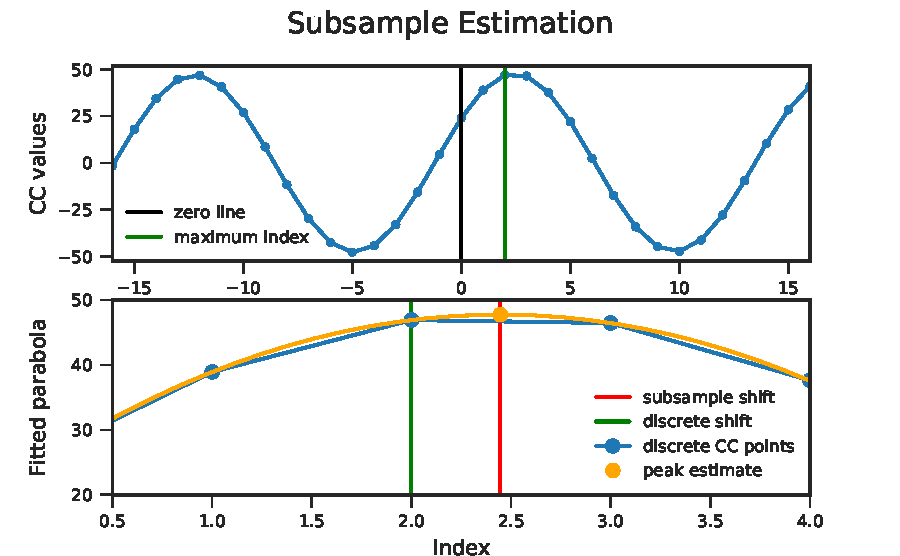
\includegraphics[]{figures/subsample_shift}
	\caption{Explanation example of the subsample shift estimation using parabolic interpolation.}
    \label{fig:02_subsampleShift}
\end{figure}
% -------------------------------------------------------------